\section{Wstęp teoretyczny}

\subsection{Procesor graficzny}
Procesory graficzne są specjalnym rodzajem procesorów,
pierwotnie stworzonych do akceleracji obliczeń graficznych.
Obliczenia te charakteryzują się dużą liczbą względnie prostych, podobnych operacji,
które mogą być przeprowadzone równolegle.
Taki model obliczeń nosi nazwę SIMD (Single Instruction Multiple Data)
i oznacza równoległe wykonywanie tej samej operacji dla wielu różnych danych wejściowych.
Współczesne karty graficzne są zaprojektowanie do wykorzystania
ich możliwości równoległych obliczeń w znacznie szerszym obszarze niż
pierwotny cel akceleracji grafiki komputerowej.
Technologie \textit{OpenCL} oraz \textit{CUDA} umożliwiają
programowanie GPGPU (\textit{general purpose GPU}) w
dziedzinach takich jak obliczenia naukowe, machine learning czy kryptografia.

\par
W mojej pracy, w celu przeprowadzenia ataku na krzywą eliptyczną, wykorzystałem
algorytm \textit{Rho Pollard'a}, który z niewielkimi modyfikacjami można bardzo skutecznie wykonywać
równolegle. Z tego powodu wykorzystanie GPU do kryptoanalizy, pozwala znacznie przyśpieszyć czas
obliczeń. W celu stworzenia programu na GPU wykorzystałem technologię Nvidia CUDA, głównie ze względu
na znacznie lepiej rozwinięty ekosystem oraz dostępność materiałów w internecie.
Standard OpenCL w przeciwieństwie do CUDA, jest tworzony na zasadach \textit{open-source} oraz może zostać
wykorzystany do programowania kart graficznych innych producentów. Niestety jest zauważalnie
gorzej wspierany w przypadku kart graficznych Nvidia.
\par
\subsubsection{Model programowania CUDA}
Program napisany w CUDA, składa się z jednego lub więcej  \\
\textit{kernel'a} - funkcji programu, która będzie się wykonywać równolegle na GPU, na każdym z uruchomionych wątków.
Wątki są grupowane w \textit{bloki}, które mogą się składać z 1 do 1024 wątków w przypadku \textit{CUDA 7.5} \cite{CudaDeveloper}.
Następnie bloki są uruchamiane na dostępnych \b{SM} - \textit{streaming multiprocessor}.
Karty graficzne Nvidia składają się zazwyczaj z kilkunastu SM, które mogą równocześnie uruchomić wiele
bloków, co pozwala na równoczesne wykonywanie kilkuset wątków.
Wątki w ramach jednego bloku dzielą pamięć współdzieloną \textit{shared memory} oraz wykonują się równocześnie.
Możliwe jest uruchomienie znacznie większej ilości bloków, niż może się jednocześnie wykonywać na dostępnych SM.
W takiej sytuacji niektóre bloki będą oczekiwać na wolne zasoby aż poprzednie nie zakończą pracy.
Dodatkowo, wątki w ramach bloku wykonują tą samą instrukcję w grupach po 32,
nazywanych \textit{warp'ami}.
W przypadku architektury SIMD ważne jest unikanie długich segmentów
warunkowych, ponieważ skutkuje to sekwencyjnymi obliczeniami.
W sytuacji gdy następuje rozgałęzienie kodu - \textit{branching},
część wątków w warp'ie musi czekać na pozostałe, skutkując sekwencyjnym wykonywaniem kodu.
Jest to szczególnie istotne dla wydajności działania programu na GPU.
\subsubsection{Hierarchia pamięci}
Kolejnym ważnym elementem który mocno wpływa na wydajność
programu, jest odpowiedni dostęp do pamięci.
Tak samo jak w zwykłym procesorze, GPU ma kilka warstw
pamięci które różnią się rozmiarem oraz czasem dostępu.
W CUDA można wyróżnić 3 najważniejsze warstwy pamięci:
\begin{itemize}
    \item Rejestry - najszybszy rodzaj pamięci, dostępny w ramach pojedynczego wątku.
          Ilość rejestrów dla każdego wątku jest jednak mocno ograniczona w przypadku
          uruchomienia wielu wątków równocześnie. Jeżeli program używa wiecej rejestrów niż jest dostępne,
          może wystąpić \textit{register spilling}, który wprowadza znaczne opóźnienia.
    \item \textit{Shared memory} - szybka pamięć współdzielona, która jest wspólna dla wątków w danym bloku. Jest ona ograniczona
          przez ilość pamięci w SM, na karcie graficznej z CUDA 7.5 jej rozmiar wynosi 64 KB \cite{CudaDeveloper}.
          Stosowana jest w przypadku, gdy wiele wątków musi się ze sobą komunikować lub w celu cache'owania danych
          i ograniczenia dostępu do znacznie wolniejszej pamięci globalnej.
          Zbyt duży rozmiar wykorzystywanej pamięci współdzielonej ogranicza ilość bloków które mogą jednocześnie się
          wykonywać na jednym SM.
    \item \textit{Global memory} - pamięć globalna DRAM, najwolniejsza oraz największa ze wszystkich warstw. Wykorzystywana głównie w celu
          komunikacji karty graficznej z procesorem, w celu przesyłania danych do obliczeń oraz zapisu wyników.
\end{itemize}
Dostępne są również dodatkowe rodzaje takie jak \textit{texture memory} oraz \textit{constant memory},
które różnią się optymalnym sposobem dostępu, jednak nie są wykorzystywane w tej pracy.

\subsection{Krzywe eliptyczne}
Zakładając, że ciało $\mathbb{K}$ ma charakterystykę różną od 2 i 3,
oraz że stałe $a, b \in \mathbb{K}$ spełniają warunek:
\[4a^3 + 27b^2 \neq 0\]
nieosobliwą krzywą eliptyczną nad ciałem $\mathbb{K}$ definiuje się jako zbiór punktów $(x,y) \in \mathbb{K} \times \mathbb{K}$,
spełniających równanie:
\[y^2 = x^3 + ax + b\]
wraz ze specjalnym punktem w nieskończoności $\mathcal{O}$, który pełni rolę elementu neutralnego
w działaniach grupowych
\cite{Stinson2021}.
\begin{figure}[H]
    \centering 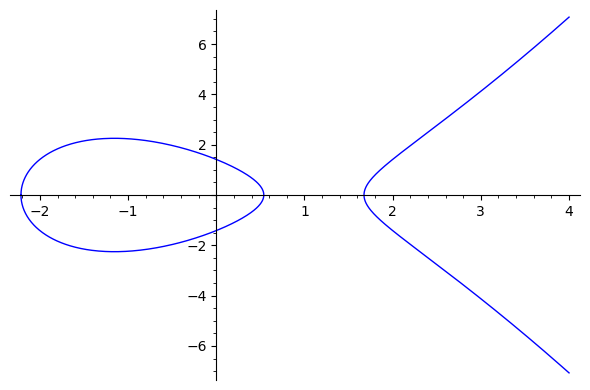
\includegraphics[width=0.8\linewidth]{sage/krzywa_-4_2.png}
    \caption{Krzywa eliptyczna $y^2=x^3-4+2$ nad ciałem liczb rzeczywistych}
\end{figure}

Krzywe eliptyczne zdefiniowane na liczbach rzeczywistych nie są kluczowe w
systemach kryptograficznych \cite*{Stinson2021}, ale takie ustawienia
pozwalają na prostsze przedstawienie niektórych zagadnień
np. dodawnie punktów na krzywej.


\subsubsection{Dodawanie punktów na krzywej eliptycznej}
Odpowiednie zdefiniowanie operacji dodawania punktów na krzywej eliptycznej
pozwala otrzymać grupę abelową, złożoną z punktów krzywej oraz punktu w nieskończoności jako
elementu neutralnego.
\newline
\indent
Geometrycznie, dodawanie punktów na krzywej eliptycznej nad ciałem liczb rzeczywistych można przedstawić
jako połączenie dwóch punktów $P$ i $Q$ prostopadłą linią, która przecina krzywą w trzecim
punkcie, $R'$. Następnie, wynikowy punkt $R$, będący sumą $P+QP+Q$, znajdujemy przez
odbicie punktu $R'$ względem osi $x$. W przypadku podwojenia punktu, czyli dodawania
punktu P do siebie samego, rysujemy styczną do krzywej w punkcie $P$, która przecina
krzywą w nowym punkcie. Odbicie tego punktu względem osi $x$ daje nam wynik $2P$ \cite{Algorytmy}\cite{Stinson2021}.
\begin{figure}[!h]
    \centering 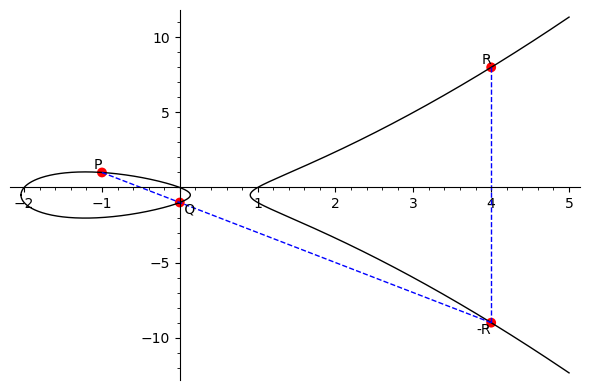
\includegraphics[width=0.8\linewidth]{sage/elliptic_rational_point_addition.png}
    \caption{P + Q na krzywej eliptycznej $y^2+y=x^3-x^2+2x$}
\end{figure}
\par
Definiując dodawanie punktów na krzywej eliptycznej w sposób algebraiczny otrzymujemy następujące wzory:
\begin{enumerate}
    \item Przypadek, gdy \( P \neq Q \):
          \begin{align}
              \lambda & = \frac{y_2 - y_1}{x_2 - x_1}, \\
              x_3     & = \lambda^2 - x_1 - x_2,       \\
              y_3     & = \lambda(x_1 - x_3) - y_1
          \end{align}
    \item Przypadek, gdy \( P = Q \):
          \begin{align*}
              \lambda & = \frac{3x_1^2 + a}{2y_1}, \\
              x_3     & = \lambda^2 - 2x_1,        \\
              y_3     & = \lambda(x_1 - x_3) - y_1
          \end{align*}
    \item Szczególny przypadek, gdy \( P = -Q \):
          \begin{align*}
              P + (-P) = \mathcal{O}
          \end{align*}
\end{enumerate}
Dodatkowo odwrotność punktu na krzywej $P$ definiujemy jako $-P = (x, -y)$ \cite{Stinson2021}.


\subsubsection{Krzywe eliptyczne na ciele skończonym}
Krzywe eliptyczne zdefiniowane na ciele skończonym $F_p$ oraz $F_{p^n}$ mają kluczowe znaczenie w kryptografii.
W swojej pracy skupiłem się wyłącznie na krzywych zdefiniowanych na ciele skończonym $F_p$ gdzie $p$ jest liczbą pierwszą.
\par
Wykres krzywej eliptycznej nad ciałem $F_p$ nie przypomina krzywej zdefiniowanej na liczbach rzeczywistych.
Krzywa taka składa się z dyskretnych punktów, których współrzędne należą do ciała
na którym jest opisana.
Operacje na krzywej nad ciałem skończonym są zdefiniowane
za pomocą tych samych wzorów algebraicznych, co w przypadku ciała liczb rzeczywistych,
jednak wszystkie działania są wykonywane na ciele $F_p$.
\begin{figure}[!h]
    \centering 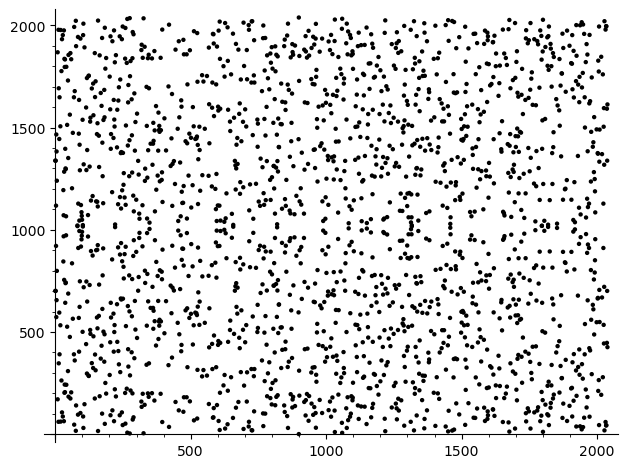
\includegraphics[width=0.8\linewidth]{sage/ec_2_11-9.png}
    \caption{Krzywa eliptyczna $y^2=x^3-4+2$ nad $GF(2^{11} - 9)$}
\end{figure}


\subsubsection{Problem logarytmu dyskretnego}
Problem logarytmu dyskretnego (\textbf{DLP}) jest
podstawą kryptosystemów oparych o grupy.
Jednymi z bardziej znanych są kryptosystem ElGamala oraz protokół wymiany
kluczy Diffie-Hellmana'a.
\\ Problem logarytmu dyskretnego można zdefiniować na grupach cyklicznych.
zarówno na grupie multiplikatywnej $(\mathbb{G},\cdot)$
oraz grupie addytywnej $(\mathbb{G}, +)$, przy odpowiednim zdefiniowaniu działań grupowych.

Jeżeli G jest grupą cykliczną a $\gamma$ jej generatorem, to logarytmem dyskretnym
elementu $\alpha \in G$ nazywamy najmniejszą nieujemną liczbę całkowitą $x$ taką, że:
\[x = \log_{\gamma}{\alpha}\]

Uważa się, że problem logarytmu dyskretnego jest trudny, ponieważ nie istnieje
algorytm, który znajduje $x$ w czasie wielomianowym\cite{Stinson2021}.


\subsubsection{Problem logarytmu dyskretnego na krzywej eliptycznej}
W przypadku krypografii opartej o krzywe eliptyczne, DLP dotyczy cykliczej \\
grupy addytywnej $(\mathbb{E},+)$ zdefiniowanej na krzywej eliptycznej.
Aby utworzyć taką grupę, wybieramy punkt $P$ na krzywej eliptycznej $\mathbb{E}$,
który będzie generatorem grupy. Wtedy grupa addytywna $\mathbb{E}$ jest generowana przez
kolejne \textit{potęgi} punktu $P$:
\[\ \langle P \rangle = \{P, 2P, 3P, \ldots, nP = \mathcal{O}\}\]
W takim przypadku, ponieważ operacją na grupie jest dodawanie modulo n, to działanie
potęgowania przedstawia się jako zwielokrotnienie punktu $P$:
\[x \cdot P = Q \textrm{ (mod } n)\]
Analogicznie do problemu logarytmu dyskretnego na grupach multiplikacyjnych,
problem logarytmu dyskretnego na krzywej eliptycznej polega na znalezieniu
$x$.
\par
Przy odpowiednim wyborze grupy addytywnej, rozwiązanie problemu logarytmu dyskretnego,
tj. znalezienie $x$,
jest trudne \cite{Stinson2021}.


\subsection{Algorytm Rho Pollard'a}

Zaproponowany przez Johna Pollard'a w 1978 roku \cite{Pollard1978},
algorytm Rho Pollard'a opiera się na wykorzystaniu paradoksu dnia urodzin w celu znalezienia logarytmu dyskretnego.
Pozwala on na znalezienie rozwiązania w czasie $O(\sqrt{n})$,
jednak jest to jedynie czas \textit{oczekiwany}, ze względu na losową naturę algorytmu \cite{Blake2005}.
W porównaniu do innego znanego algorytmu, Baby-Step Giant-Step \cite{Stinson2021}, algorytm Rho Pollard'a jest bardziej
efektywny pamięciowo, nie wymagając
przestrzeni $O(\sqrt{n})$ a jedynie $O(1)$ w wersji sekwencyjnej \cite{Stinson2021}\cite{Blake2005}.
\par

Idea algorytmu polega na losowym błądzeniu po krzywej eliptycznej
w celu znalezienia kolizji dwóch punktów, które spełniają równanie:
$$
    a P + b Q = a' P + b' Q \textrm{ (mod } n)
$$
gdzie $P$ jest generatorem grupy cyklicznej rzędu $n$ na krzywej eliptycznej $\mathbb{E}$ \\
oraz $x \cdot P = Q$, więc $x$ jest szukanym rozwiązaniem problemu.
Gdy znajdziemy kolizję, odpowiednio przekształcając powyższe równanie, możemy znaleźć
$x$:
$$
    x \equiv \frac{(a-a')}{(b'-b)} \textrm{ (mod } n)
$$


Klasyczny algorytm Rho Pollard'a, oparty o poszukiwanie cyklu,
aby znaleźć kolizję, iteracyjne oblicza parę trójek:
$(R_i,a_i,b_i)$ oraz $(R_j,a_j,b_j)$ gdzie $R_j, R_i \in \mathbb{E}$, które spełniają
własność $R = a P + b Q$:
$$
    f(R,a,b) =
    \begin{cases}
        (R + P,a,b+1)     & \text{if } R \in S_1, \\
        (2R,2a, 2b)       & \text{if } R \in S_2, \\
        (R + Q, a + 1, b) & \text{if } R \in S_3,
    \end{cases}
$$
$S_1 \cup S_2 \cup S_3$ jest podziałem $\mathbb{E}$ na trzy podzbiory, które powinny być podobnej wielkości.
Ponieważ $R$ jest punktem na krzywej eliptycznej a nie liczbą całkowitą, często stosowanym sposobem
podziału różnych wartości $R$ na trzy zbiory, jest obliczanie operacji modulo $3$ ze współrzędnej $x$.
Aby z kolejno obliczanych trójek znaleźć kolizję punktów, często stosuje się algorytm poszukiwania cyklu Floyd'a.
W takim przypadku, obliczamy w każdej iteracji obliczamy trójki: $(R_i, a_i, b_i)$ oraz $(R_{2i}, a_{2i}, b_{2i})$, aż do znalezienia
kolizji $R_i = R_{2i}$.

\par
Sekwencyjna wersja algorytmu słabo się skaluje w przypadku zwiększania ilości równolegle działających procesorów,
osiągając jedynie przyśpieszenie rzędu $O(\sqrt{m})$ dla $m$ procesorów \cite{Oorschot}.
Dlatego w swojej pracy wykorzystałem równoległą wersję algorytmu, zaproponowaną przez Van Oorschota i Wienera \cite{Oorschot}.

\subsubsection{Równoległy algorytm Rho Pollarda}
Równoległa wersja algorytmu Rho Pollard'a, zakłada zastosowanie wielu równolegle działających
procesorów, które niezależnie od siebie wykonują \textit{spacer losowy} po krzywej eliptycznej,
w poszukiwaniu \textit{punktów wyróżnionych}. Gdy znajdą taki punkt, przekazują go do serwera centralnego,
który odpowiada za gromadzenie znalezionych punktów wyróżnionych oraz poszukiwanie kolizji między nimi.
\par
Cecha określająca czy dany punkt na krzywej jest wyróżniony, powinna być łatwo weryfikowalna i tania obliczeniowo,
ponieważ sprawdzenie czy dany punkt jest wyróżniony, występuje w każdej iteracji algorytmu. \\
Często wybieranym sposobem sprawdzenia czy punkt jest wyróżniony, jest obliczenie ilości zer na początku lub na końcu
reprezentacji bitowej jednej ze współrzędnych punktu. Różny dobór tej cechy wpływa na pamięć oraz
czas wymagany do znalezienia kolizji. Bardzo szeroki zakres punktów które spełniają kryteria bycia wyróżnionymi,
spowoduje bardzo szybkie zapełnienie pamięci centralnego serwera a za wąski spowoduje, że czas do znalezienie kolizji się wydłuży.

\subsubsection{Adding Walk}

Adding Walk jest modyfikacją funkcji iteracyjnej $f$ używanej w algorytmie Pollard’s 
Rho do obliczania kolejnych punktów na krzywej eliptycznej. Funkcja ta opiera się 
na dodawaniu w każdej iteracji punktów z predefiniowanej tablicy punktów, co 
zapewnia wysoką efektywność oraz równomierny rozkład iteracji w grupie. Wprowadzenie 
Adding Walk, jak pokazano w pracy Teske \cite{Teske2000}, poprawia wydajność w 
stosunku do oryginalnej wersji algorytmu, zapewniając prostszą implementację w 
przypadku równoległych obliczeń, takich jak te wykonywane na GPU.

Niech $W_0 = nP$ będzie punktem startowym, gdzie $n$ to znana wielokrotność 
generatora grupy $P$. Funkcja iteracyjna $f$ jest zdefiniowana jako odwzorowanie 
$f: \langle P \rangle \rightarrow \{1, \ldots, s\}$ o możliwie równomiernym 
rozkładzie. Następnie definiujemy tablicę predefiniowanych punktów:
$$
R_i = c_i P + d_i Q, \quad \text{dla } 0 \leq i \leq s - 1,
$$
gdzie $c_i$ i $d_i$ są współczynnikami losowymi. Funkcja iteracyjna jest zdefiniowana 
jako:
$$
W_{i+1} = W_i + R_{f(W_i)}.
$$
Podczas każdej iteracji konieczne jest zliczanie współczynników odpowiadających 
wielokrotnościom $P$ i $Q$, aby każdy punkt na krzywej mógł zostać jednoznacznie 
przedstawiony w postaci $aP + bQ$. Suma współczynników $a$ i $b$ jest aktualizowana 
w każdej iteracji zgodnie z wartościami predefiniowanych współczynników 
$c_i$ i $d_i$ dla punktu $R_{f(W_i)}$. Zliczanie tych wartości jest kluczowe 
dla odtworzenia obliczeń w przypadku znalezienia kolizji, umożliwiając późniejsze 
wyznaczenie logarytmu dyskretnego.

Istotnym czynnikiem jest również rozmiar tablicy $s$, który ma spore znaczenie
dla skuteczności algorytmu. Zbyt mała 
wartość $s$ może powodować, że funkcja iteracyjna nie będzie wystarczająco 
"losowa". Eksperymenty wykazały, że dla $s \geq 16$, funkcja $f$ zapewnia 
odpowiedni poziom losowości, niezależnie od rozmiaru grupy \cite{Teske2000}.

Główną zaletą tej metody w implementacjach GPU jest minimalizacja rozgałęzień 
w czasie iteracji. Dzięki temu niemal wszystkie wątki wykonują tę samą operację 
dodawania punktów, co jest istotne w architekturze SIMD (Single Instruction, 
Multiple Data). Wyjątkiem jest rzadki przypadek, gdy $W_i = R_{f(W_i)}$, co 
wymaga wykonania operacji zwielokrotnienia punktu.
